%************************************************
%\chapter{Trends in CO$_2$ flux} % $\mathbb{ZNR}$
\chapter{Processes corresponding to multi-year sea-air CO$_2$ flux trends}
%************************************************
\label{ch:trends}

%\section[Winds determine internal variability]{Winds determine internal variability of the Southern Ocean CO$_2$ flux}
%\section[Westerly winds and Southern Ocean CO$_2$ flux variability]{The role of westerly winds on Southern Ocean CO$_2$ flux variability}
\section{The role of westerly winds in Southern Ocean CO$_2$ flux variability}

%\paragraph{on area 50-60S as driver of Southern Ocean internal variability, correlation plots co2flux and wind trends} 
\cite{Thompson2000} and \cite{Hall2002} describe the \ac{SAM} as the most dominant mode for higher-latitude Southern Hemisphere variability. \cite{Lovenduski2007} explains the influence of the westerly winds on the Southern Ocean carbon sink. To further assess internal variability due to westerly winds, this chapter discusses the effect of westerly winds on the physical and biological controls of the Southern Ocean carbon sink in \acs{HAMOCC}.\newline

I find a correlation on 8-year trends between \acs{SAM}, which describes the position and latitudinal shift of westerly winds, and the CO$_2$ flux in the area of largest decadal internal variability at 50-60$^\circ$S (fig. \ref{fig:scatter}). Although the CO$_2$ flux formula (see section \ref{sec:HAMOCC}) depends on the wind speed at 10m height, the importance and the changes in figure \ref{fig:scatter} are not in the piston velocity $k_w$ but in $\Delta \text{pCO}_2$ \citep{Lovenduski2015}. However, the magnitude of short-term variability on the timescale of days to hours depends highly on wind strength variability, but the direction of CO$_2$ flux is independent of wind speed. This relationship reveals two distinct regimes of wind-driven CO$_2$ flux signals in this area: 

Intensified and southward shifted winds, associated with an increasing trend in \acs{SAM}, lead to a positive CO$_2$ flux trend. This Southern Ocean carbon sink response has been suggested frequently for the observed and projected trend in \acs{SAM} \citep{LeQuere2007,Lovenduski2007,Lovenduski2008,Hauck2013}. The related processes associated stronger winds are explained in section \ref{sec:trends_pos}.

In \acs{MPI-ESM}, I also find the reverse case of weakening and northward shifting winds, associated with a negative trend in \acs{SAM}, which lead to a negative CO$_2$ flux or ocean uptake trend. The related processes associated with weaker winds are explained in section \ref{sec:trends_neg}. However, observations do not reveal strong multi-year negative \acs{SAM} trends (see fig. \ref{fig:evolution_SAM}). Likewise, westerly winds did not weaken, but continued to increase during the negative CO$_2$ flux trend in the 2000s \citep{landschuetzer2015}. On the contrary, depending on the starting year of the trend period, the \acs{SAM} index slightly weakened in the early 2000s \citep{Marshall2003,Lovenduski2015}. \newline

The strong trends originate in strong changes of the position and strength of Southern hemisphere westerly winds and effect of those on ocean circulation. However, the parametrized eddies in \acs{MPI-ESM LE} might allow deeper mixing to sustain for multiple years and hence longer than the seasonal timescale at which the eddies would counteract those trends \citep{Thompson2011}. Only a variable definition of isopyncal thickness diffusion could parametrize the expected eddy response from high-resolution simulations \citep{Gent2011}. These enhanced eddy fluxes in a low-resolution model are discussed in \cite{Lovenduski2013}.


\begin{figure}[h!]
\centering
%		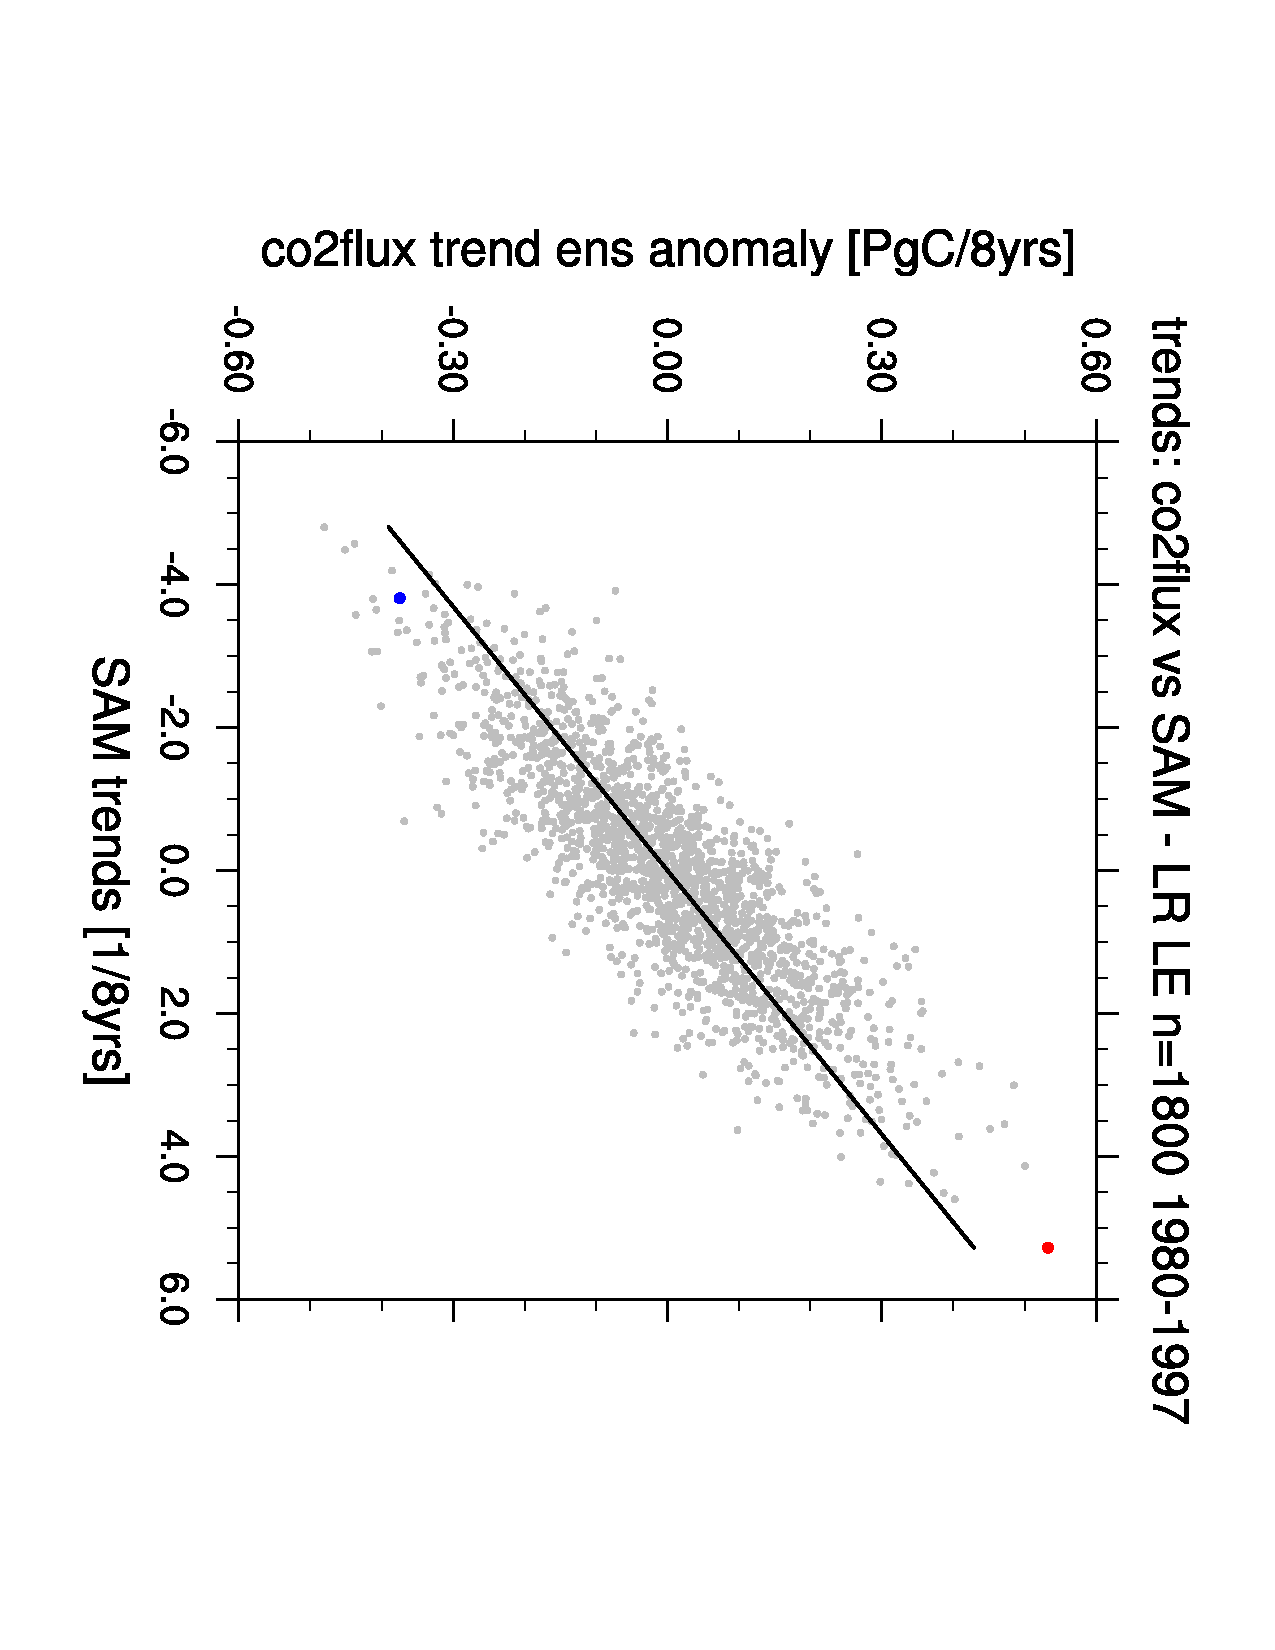
\includegraphics[scale=.5,page=1,angle=90,trim=1.3cm 2.3cm 2.3cm 3cm,clip]{Scatter_trends_bands_ensanom_co2flux_vs_SAM_n1800_1980_1997_trend8_50-59S}
		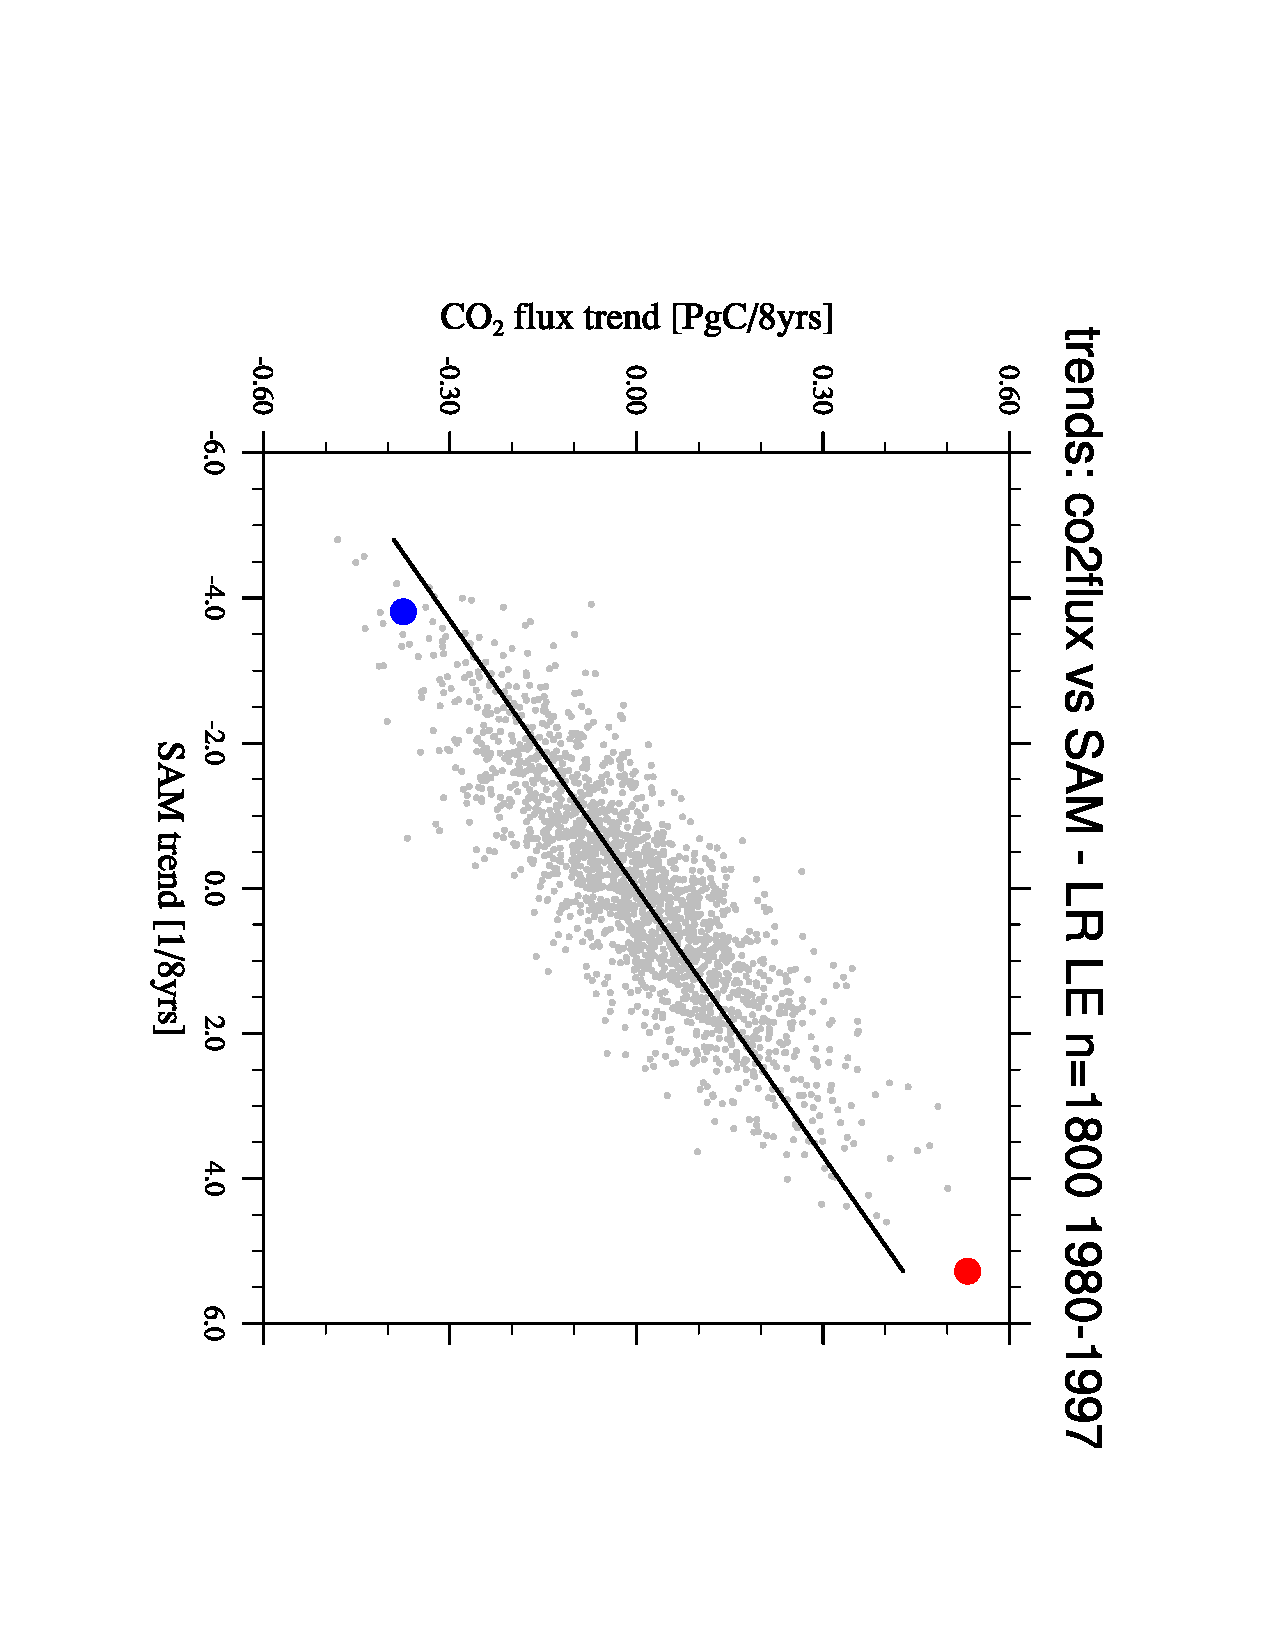
\includegraphics[scale=.6,page=1,angle=90,trim=1.3cm 2.3cm 3.8cm 4cm,clip]{EGU_new_SAM_Scatter_trends_bands_ensanom_co2flux_vs_SAM_n1800_1980_1997_trend8}
		
		%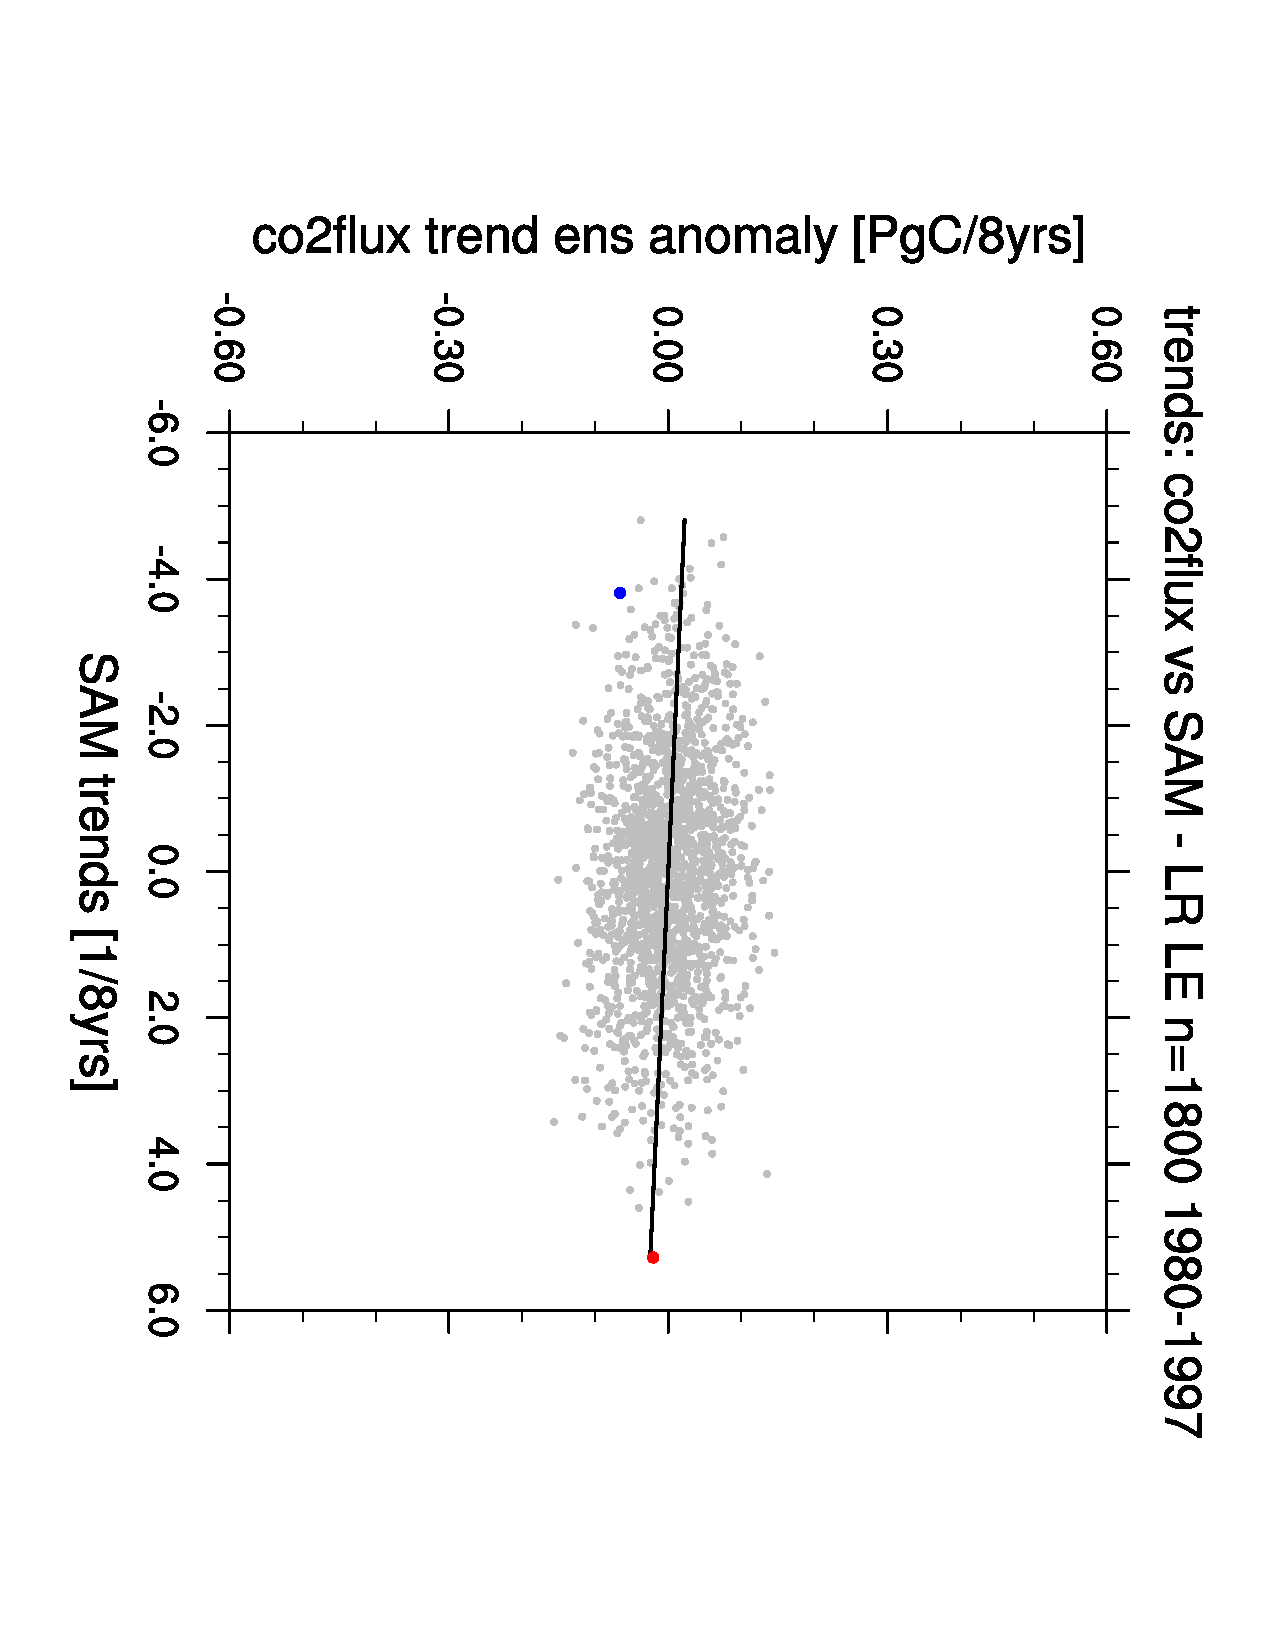
\includegraphics[scale=.38,page=1,angle=90,trim=1.3cm 2.3cm 2.3cm 3cm,clip]{Scatter_trends_bands_ensanom_co2flux_vs_SAM_n1800_1980_1997_trend8_40-49S}
		\vspace{-2mm}
		\caption{Linear trends in the \ac{SAM} as indicator of wind strength vs. CO$_2$ flux at 50-60$^\circ$S; each data point represents 8-year trends of a single realization normalized for the ensemble mean trend  between 1980 and 2004; the blue dot is the most negative monotonic CO$_2$ flux trend; the red dot is positive monotonic CO$_2$ flux trend.}
		\label{fig:scatter}
\end{figure}

To qualitatively understand the mechanisms of the Southern Ocean carbon sink, I analyze the drivers of CO$_2$ flux on a process level. This chapter covers CO$_2$ flux changes with respect to the thermal effect, physical circulation and biology. A quantitative analysis of the different drivers for different regions discussed in chapter \ref{ch:pCO2separation}.

The analysis presented here involves 8-year trends for reasons stated in section \ref{sec:choicetrend}, but the results of this chapter apply to various multi-year trends subject to internal variability (not shown).

The spatial trend patterns of different trend periods appear zonally symmetric, therefore the analysis is not separated into the different Southern Ocean sectors, e.g. Pacific, Indian or Atlantic. Also, the atmospheric circulation change in models are too symmetric compared to observations \citep{Haumann2014}. Therefore, the description here is carried out in zonal latitudinal bands keeping the unsymmetrical Southern Ocean dynamics in mind \citep{Sallee2010,Talley2013}. Also due to the underestimated Antarctic sea-ice and open-ocean convection in the Ross and Weddell Sea, I restrict my analysis to the Southern Ocean north of 60$^\circ$S, but the decadal CO$_2$ flux trends have a weak signal south of 60$^\circ$S anyway. 



\clearpage

\section{Positive CO$_2$ flux trends}
\label{sec:trends_pos}

Strong positive CO$_2$ flux trends correlate with stronger westerly winds (fig. \ref{fig:scatter}) \citep{Lovenduski2007}. The difference $\Delta$pCO$_2$ between oceanic pCO$_{2,\text{ocean}}$ and atmospheric partial pressures pCO$_{2,\text{atm}}$ depicts a cleaner signal than CO$_2$ flux and is independent of wind speed and solubility \citep{Lovenduski2015}. pCO$_{2,\text{ocean}}$ rises stronger than pCO$_{2,\text{atm}}$, so CO$_2$ must be driven by changes in the ocean dynamics (fig. \ref{fig:pco2_pos}a).
The strongest positive signal occurs in the upwelling at 50-60$^\circ$S, a weaker and more patchy signal occurs in the subduction areas north of 50$^\circ$S, whereas changes in most other areas of the Southern Ocean are insignificant (fig. \ref{fig:pco2_pos}a). 

Westerly winds decrease at 40-50$^\circ$S and increase at 50-60$^\circ$S which results in a southward shift of westerlies (fig. \ref{fig:pco2_pos}b) represented by the positive trend in \acs{SAM} (see fig. \ref{fig:evolution_SAM}). \newline


The response of the thermal effect, upper-ocean overturning circulation and biology are described in sections \ref{sec:trends_pos_thermal}, \ref{sec:trends_pos_circulation} and \ref{sec:trends_pos_biology}, respectively.


\begin{figure}[h!]
\centering
	\topinset{(a)}{\includegraphics[scale=.57,trim=6.3cm 14.4cm 5.5cm 6.4cm,clip]{\memberpositive _positive_trend_8_Landschuetzer_overview.pdf}}{0.02in}{.02in}
	\topinset{(b)}{\includegraphics[scale=.75,trim=7.2cm 4.7cm 6.8cm 17.8cm,clip]{\memberpositive _positive_trend_8_Landschuetzer_overview.pdf}}{0.02in}{.02in}
	\caption{Linear trends in $\Delta$pCO$_2$ (a) and \ac{SLP} and wind vectors overlain as arrows (b) for the case of the most positive monotonic 8-year CO$_2$ flux trend; hatched areas indicate where trends are outside the 5\% significance level}% - should I also discuss thermal and non-thermal trends in \citep{landschuetzer2015}?}
	\label{fig:pco2_pos}
\end{figure}






\clearpage

\subsection{Changes in the thermal effect during positive CO$_2$ flux trends}
\label{sec:trends_pos_thermal}

The difference between the partial pressure of CO$_2$ in oceanic pCO$_{2,\text{ocean}}$ and atmospheric pCO$_{2,\text{atm}}$ is the main changing quantity in the CO$_2$ flux formula. The separation by \cite{Takahashi2002} gives insights about the direct influence of \ac{SST} (see section \ref{sec:takahashi}). The thermal pCO$_2$ trend is driven by changes in \acs{SST} (fig. \ref{fig:thermal_pos}a), whereas the non-thermal trend includes changes in pCO$_{2,\text{atm}}$, biology, alkalinity, at constant \acs{SST} (fig. \ref{fig:thermal_pos}b). The thermal pCO$_2$ trend and non-thermal $\delta pCO_2$ trend approximately add up to the trends in pCO$_2$ \citep{landschuetzer2015}.

The thermal trend follows the \acs{SST} cooling trend (fig. \ref{fig:sst_pos}) south of 50$^\circ$S towards negative CO$_2$ flux trends, whereas the warming north of 50$^\circ$S favors outgassing. Increased Ekman transport causes this heat divergence in polar regions and a heat convergence at lower latitudes \citep{Hall2002} (see fig. \ref{fig:UOOC_pos}). The non-thermal component strongly increases south of 50$^\circ$S, so overall the pCO$_{2,\text{ocean}}$ increases faster than pCO$_{2,\text{atm}}$, which leads to a positive CO$_2$. This reflects the enhanced outgassing from increased upwelling. The non-thermal and thermal trends combined nearly compensate north of 50$^\circ$S, but at 50-60$^\circ$S the outgassing dominates (fig. \ref{fig:pco2_pos}a). The homogenous increase in atmospheric pCO$_{\text{2,atm}}$ accounts for a -12ppm/8yrs in fig. \ref{fig:pco2_pos}b. 
These changes are stronger in the summer season, especially the non-thermal component (see fig. \ref{fig:thermal_pos_summer}, \ref{fig:thermal_pos_winter}). 

\begin{figure}[h!]
\centering
	\topinset{(b)}{\topinset{(a)}{\includegraphics[scale=1.22,trim=6.25cm 10.2cm 5.2cm 14cm,clip]{\memberpositive _positive_trend_8_Landschuetzer_overview.pdf}}{0.03in}{.02in}}{.03in}{2.in}
	\caption{Linear trends in pCO$_{2,\text{thermal}}$ (a) and $\Delta$pCO$_{2,\text{non-thermal}}$ (b) for the case of the most positive monotonic 8-year CO$_2$ flux trend; hatched areas indicate where trends are outside the 5\% significance level}
	\label{fig:thermal_pos}
\end{figure}



\clearpage

\subsection{Changes in ocean circulation during positive CO$_2$ flux trends}
\label{sec:trends_pos_circulation}

Stronger westerly winds intensify the upper-ocean overturning circulation \citep{Lauderdale2013}. The circulation field advects \acs{DIC} along its overturning pathway (fig. \ref{fig:UOOC_pos}). Intensified upwelling of carbon-rich waters 50-60$^\circ$S increases \acs{DIC} concentrations in the euphotic zone (fig. \ref{fig:ekman_pos}b). An over-saturation in \acs{DIC} leads to a positive CO$_2$ flux. The stronger winds also increase Ekman northward transport and advects \acs{DIC} further northward (fig. \ref{fig:ekman_pos}a). North of 50$^\circ$S, subduction rates of \ac{AAIW} and \ac{SAMW} formation increase, so pCO$_{2,\text{atm}}$-equilibrated waters take additional anthropogenic carbon into the deeper ocean. The southward shift of westerly winds weakens the northern edge of Ekman transport at 30-40$^\circ$S. 

The changes in \ac{MLD} also contribute to the vertical transport of carbon. By deeper mixing in winter, more carbon-rich waters are included in the \acs{MLD}, which then serves as a larger reservoir of super-saturated \acs{DIC}. \acs{MLD} deepens south of 50$^\circ$S and slightly shoals north of 45$^\circ$S, whereas open-ocean convection causes the unrealistic zonal \acs{MLD} averages below 300m south of 60$^\circ$S (fig. \ref{fig:UOOC_pos}) \citep{Sallee2013,Stoessel2015}. 


\begin{figure}[h!]
	\centering
	\topinset{(a)}{\includegraphics[scale=1.07,trim=13.cm 18.75cm 3cm 6cm,clip]{\memberpositive _positive_trend_8_ekman_overview.pdf}}{0.16in}{.09in}
	\topinset{(b)}{\includegraphics[scale=1.07,trim=13.25cm 15.9cm 3cm 9.2cm,clip]{\memberpositive _positive_trend_8_ekman_overview.pdf}}{0.in}{.0in}
	\vspace{-5mm}
	\caption{Linear trends in Ekman transport (a) and Ekman pumping (b) in the case of the most positive 8-years CO$_2$ flux trend; hatched areas indicate where trends are outside the 5\% significance level}
	\label{fig:ekman_pos}
\end{figure}


\begin{figure}[h!]
	\centering
	\includegraphics[scale=0.42,page=2,trim=.3cm 1.7cm 0cm 4.6cm,clip]{UOOC}
	\vspace{-5mm}
	\caption{Zonally averaged upper-ocean overturning circulation in the case of the most positive 8-year CO$_2$ flux trend; black arrows show mean advective carbon transport, red arrows show advective carbon transport trends enforcing the upper-ocean overturning circulation; blue arrows show advective carbon transport trends weakening the upper-ocean overturning circulation; black numbers quantify the trends in advective carbon transport in PgC/8yrs; white lines are isopyncals as in fig. \ref{fig:UOOC_mean}; grey line is \ac{MLD} in the beginning and the black line MLD in the end of the period.}
	\label{fig:UOOC_pos}
\end{figure}

The upper-ocean overturning circulation response presented here is in line with idealized wind-change studies \citep{Lauderdale2013}, modeling studies explaining the observed CO$_2$ flux trend in the 1990s \citep{LeQuere2007,Lovenduski2007,Lovenduski2008}, as well an inverse modeling study for the 1990s \citep{DeVries2017}.


\clearpage

\subsection{Changes in biology during positive CO$_2$ flux trends}
\label{sec:trends_pos_biology}
The biological pump draws down surface \ac{DIC} and is sensitive to changes in circulation (see section \ref{sec:HAMOCC}). In this subsection, I analyze the 8-year summer (SONDJF) austral summer trends of quantities related to primary production. 
  
Primary production and CO$_2$ flux show opposing zonally symmetric trend patterns as phytoplankton growth takes up large amounts of surface \acs{DIC} and hence lowers pCO$_2$ (fig. \ref{fig:summer_trends_pos}a,b). Primary production declines most pronounced at 50-60$^\circ$S, increases at 40-50$^\circ$S and declines at 30-40$^\circ$S. Why?
%\paragraph{on intpp not increasing because of more nutrients} different than \citep{Lovenduski2005} 


Internally varying processes change the availability of nutrients. 
The decline in nutrients in the subtropics at 30-40$^\circ$S reduces primary production, but the nutrient availability factor (for definition see \ref{sec:HAMOCC}) slightly increases south of 50$^\circ$S (fig. \ref{fig:summer_trends_pos}c).
Previous observational and modeling studies suggest an increase in primary production, because upwelling brings nutrients, especially iron, from the deep-ocean to the iron-limited surface waters \citep{Lovenduski2005,Hauck2013,wang2012,Tagliabue2014}. Additional iron fosters primary production following the iron-hypothesis \citep{Martin1990Nature,Martin1990}, but observational data for iron is still rather sparse to test this for the whole Southern Ocean \citep{Tagliabue2014}. Contrasting HAMOCC, many models reproduce this suggested iron-limitation in the Southern Ocean and hence respond with increase primary production \citep{wang2012,Hauck2013}.  \newline

If the reduction in primary production at 50-60$^\circ$S cannot be explained by changes in nutrients, what else effects primary production blooms?

The combined light \& temperature limitation is primarily driven by temperature after the insulation excels a threshold in cold waters (see fig. \ref{fig:lighttemplimf}). A strong \acs{SST} cooling trend comes along with stronger winds, because the increased Ekman transport pushes cold polar waters more northward (fig. \ref{fig:sst_pos}). The strong light \& temperature limitation signal in coastal areas as well as Weddell and Ross Sea is attributed to sea-ice changes and open-ocean convection, but has minor effects on the primary production and CO$_2$ flux (fig. \ref{fig:summer_trends_pos}d). 

This northward Ekman transport could also advect phytoplankton northwards to cause the increase in primary production at 40-50$^\circ$S (fig. \ref{fig:ekman_pos}).

The overall decline of primary production in the Southern Ocean under a positive \acs{SAM} trend is related to mixing:
The summer \ac{MLD} has a strong increasing trend at 50-60$^\circ$S, so the mixing deepens (fig. \ref{fig:summer_trends_pos}e). This is caused by stronger winds (fig. \ref{fig:pco2_pos}b) and shown in the average depth of the vertical diffusivity due to wind (fig. \ref{fig:summer_trends_pos}f). This deeper mixing in summer then mixes the standing stock of phytoplankton to deeper levels, where they are exposed to less light (fig. \ref{fig:summer_trends_pos}g) \citep{Margalef1997}. This theory of a critical depth for phytoplankton blooms was proposed by \cite{Sverdrup1953} and requires a stable water column for phytoplankton to initiate blooms. However, this theory is based on turbulent mixing, so the oceanographic \acs{MLD} only serves as a first-order mixing measure for phytoplankton \citep{Franks2014}. Still the signal sustains to phytoplankton depth, where the average phytoplankton depth decreases up to 15m which results in up to 30\% less light. The lack of monthly output for 3D biogeochemical variables made me use annual averages for phytoplankton, which causes the low significance in fig. \ref{fig:summer_trends_pos}g. 

The reverse processes contributes to the increase at 40-50$^\circ$S: Less winds mix less deep and allow phytoplankton to stay more confined to the surface, where they get more light and flourish (fig. \ref{fig:pco2_pos}b, \ref{fig:summer_trends_pos}e,f,g,b). Also the warming increases the phytoplankton growth rate (fig. \ref{fig:summer_trends_pos}d).
\\

Summarizing, a multitude of interconnected processes causes the decline in primary production in the Southern Ocean for an increasing \acs{SAM} trend. A clear separation of the magnitude of the different effects is impossible.
 
%\llap{ \parbox[b]{8.0cm}{\textbf{a}\\\rule{0ex}{3.7cm}}} %http://tex.stackexchange.com/questions/128844/put-subfigure-labels-inside-figures-using-subfig-package
%%%	\llap{ \parbox[b]{.5cm}{\textbf{b}\\\rule{0ex}{3.7cm}}}	

\begin{figure}[h!] %lbrt
%	%\topinset{(a)}{\includegraphics[scale=0.45,page=4,trim=1.4cm 1.7cm 0cm 4.6cm,clip]{UOOC}}{0.07in}{.12in}
	\topinset{(a)}{\includegraphics[scale=1.15,trim=13.2cm 18.75cm 3.4cm 6.3cm,clip]{\memberpositive _positive_trend_8_obgc_overview_summer.pdf}}{0.04in}{.01in} %co2flux
	\topinset{(b)}{\includegraphics[scale=1.15,trim=13.2cm 15.9cm 3.4cm 9.225cm,clip]{\memberpositive _positive_trend_8_obgc_overview_summer.pdf}}{0.04in}{.01in} %intpp
	\topinset{(c)}{\includegraphics[scale=1.15,trim=13.2cm 13.05cm 3.4cm 12.075cm,clip]{\memberpositive _positive_trend_8_obgc_overview_summer.pdf}}{0.04in}{.01in} %nutlimf
	\topinset{(d)}{\includegraphics[scale=1.15,trim=13.2cm 4.5cm 3.4cm 20.65cm,clip]{\memberpositive _positive_trend_8_obgc_overview_summer.pdf}}{0.04in}{.01in} %light_temp	
	\topinset{(e)}{\includegraphics[scale=1.15,trim=13.2cm 7.3cm 3.4cm 17.775cm,clip]{\memberpositive _positive_trend_8_obgc_overview_summer.pdf}}{0.04in}{.01in} %zmld
	\topinset{(f)}{\includegraphics[scale=1.15,trim=13.2cm 15.9cm 3.4cm 9.2cm,clip]{\memberpositive _positive_trend_8_schwerpunkt_mixing_overview.pdf}}{0.04in}{.01in} % wind penetration depth	
	\topinset{(g)}{\includegraphics[scale=1.15,trim=13.2cm 18.7cm 3.4cm 6.38cm,clip]{\memberpositive _positive_trend_8_schwerpunkt_mixing_overview.pdf}}{0.04in}{.01in} % phy depth	

	\caption{Southern Ocean austral summer trends for the case of the most positive 8-year CO$_2$ flux trend: CO$_2$ flux (a), vertically integrated primary production (b), nutrient availability factor (c), surface temperature \& limitation function (d), \ac{MLD} (e); average depth of vertical diffusivity due to wind (f) and phytoplankton average depth (g); hatched areas indicate where trends are outside the 5\% significance level}
	\label{fig:summer_trends_pos}
\end{figure}



\clearpage



\section{Negative CO$_2$ flux trends}
\label{sec:trends_neg}

Disclaimer: Generally, trends in this analysis reverse for weaker compared to strengthening westerlies, which leads to an overall negative CO$_2$ flux trend. Additionally, now the prescribed atmospheric $pCO_{2,\text{atm}}$ forcing promotes a steady negative background CO$_2$ flux trend.\newline

Strong negative CO$_2$ flux trends correlate with weaker westerly winds (fig. \ref{fig:pco2_neg}). The strongest negative signal $\Delta$pCO$_2$ occurs in the upwelling at 50-60$^\circ$S, whereas changes in most other areas of the Southern Ocean are insignificant (fig. \ref{fig:pco2_neg}a). 

Westerly winds decrease at 40-60$^\circ$S, which results in a northward shift of westerlies (fig. \ref{fig:pco2_pos}) represented by the negative trend in \acs{SAM} (see fig. \ref{fig:evolution_SAM}).
\\

%The strengthening of the Southern Ocean carbon sink under the context of intensified westerly winds leads me to a hypothesis (fig. \ref{fig:schematics_pos}):
%Weaker winds at 50-60$^\circ$S slow down the upper-ocean overturning circulation and increase primary production due to a more stable water column. [really unsure about this hypothesis part - I dont discover anything new but want to explain the process with a figure ahead]
The response in the thermal effect, upper-ocean overturning circulation and biology are described in sections \ref{sec:trends_neg_thermal}, \ref{sec:trends_neg_circulation} and \ref{sec:trends_neg_biology}, respectively.


\begin{figure}[h!]
\centering
%\topinset{(a)}{\includegraphics[scale=.57,trim=6.3cm 14.4cm 5.5cm 6.4cm,clip]{\memberpositive _positive_trend_8_Landschuetzer_overview.pdf}}{0.02in}{.02in}
	\topinset{(a)}{\includegraphics[scale=.57,trim=6.3cm 14.4cm 5.5cm 6.4cm,clip]{\membernegative _positive_trend_8_Landschuetzer_overview.pdf}}{0.02in}{.02in}
	\topinset{(b)}{\includegraphics[scale=.75,trim=7.2cm 4.7cm 6.8cm 17.8cm,clip]{\membernegative _positive_trend_8_Landschuetzer_overview.pdf}}{0.02in}{.02in}	
	\caption{Linear trends in $\Delta$pCO$_2$ (a) and sea-level pressure and wind vectors overlain as arrows (b) for the case of the most negative monotonic 8-year CO$_2$ flux trend; hatched areas indicate where trends are outside the 5\% significance level}
	\label{fig:pco2_neg}
\end{figure}

\clearpage

\subsection{Changes in the thermal effect during negative CO$_2$ flux trends}
\label{sec:trends_neg_thermal}

The thermal trend follows the \ac{SST} warming trend (fig. \ref{fig:sst_neg}) south of 50$^\circ$S towards positive CO$_2$ flux trends, whereas the cooling north of 50$^\circ$S favors CO$_2$ uptake (fig. \ref{fig:thermal_neg}a). This is caused by a heat convergence in the polar region and a heat divergence in the subtropics caused by less Ekman transport \citep{Hall2002}. The non-thermal trend is slightly positive north of 50$^\circ$S and negative south of 50$^\circ$S with the strongest signal in the areas of upwelling at 50-60$^\circ$S (fig. \ref{fig:thermal_neg}b). The increase in atmospheric pCO$_{\text{2,atm}}$ accounts for a -14ppm/8yrs. The non-thermal and thermal trends combined nearly compensate  north of 50$^\circ$S, but the non-thermal component dominates at 50-60$^\circ$S (fig. \ref{fig:pco2_neg}a). 

These changes are stronger in the summer season, especially the non-thermal component (see fig. \ref{fig:thermal_neg_summer}, \ref{fig:thermal_neg_winter}). 

\begin{figure}[h!]
%\centering
	\topinset{(b)}{\topinset{(a)}{\includegraphics[scale=1.22,trim=6.25cm 10.2cm 5.2cm 14cm,clip]{\membernegative _positive_trend_8_Landschuetzer_overview.pdf}}{0.03in}{.02in}}{.03in}{2.in}
	\caption{Linear trends in pCO$_{2,\text{thermal}}$ (a) and $\Delta$pCO$_{2,\text{non-thermal}}$ (b) for the case of the most negative monotonic 8-year CO$_2$ flux trend; hatched areas indicate where trends are outside the 5\% significance level}
	\label{fig:thermal_neg}
\end{figure}
 





\clearpage

\subsection{Changes in ocean circulation during negative CO$_2$ flux trends}
\label{sec:trends_neg_circulation}

Weaker westerly winds slow down the upper-ocean overturning circulation \citep{Lauderdale2013}. The circulation field advects \acs{DIC} along its overturning pathway (fig. \ref{fig:UOOC_neg}). Weaker upwelling of carbon-rich waters 50-60$^\circ$S decreases \acs{DIC} concentrations in the euphotic zone (fig. \ref{fig:ekman_neg}b). An under-saturation in \acs{DIC} leads to a negative CO$_2$ flux. Weaker winds also decrease Ekman northward transport and advects \acs{DIC} less northward (fig. \ref{fig:ekman_neg}a). North of 50$^\circ$S, subduction rates of \acs{AAIW} and \acs{SAMW} formation decrease, so pCO$_{2,\text{atm}}$-equilibrated waters take less anthropogenic carbon into the deeper ocean. The northward shift of westerly winds strengthens the northern edge of Ekman transport at 30$^\circ$S. \acs{MLD} shoals south of 50$^\circ$S and slightly deepens north of 45$^\circ$S, whereas open-ocean convection causes the unrealistic zonal \acs{MLD} averages below 300m south of 60$^\circ$S  (fig. \ref{fig:UOOC_neg}). 


\begin{figure}[h!]
	\centering
	\topinset{(a)}{\includegraphics[scale=1.07,trim=13.cm 18.75cm 3cm 6cm,clip]{\membernegative _positive_trend_8_ekman_overview.pdf}}{0.16in}{.09in}
	\topinset{(b)}{\includegraphics[scale=1.07,trim=13.25cm 15.9cm 3cm 9.2cm,clip]{\membernegative _positive_trend_8_ekman_overview.pdf}}{0.0in}{.0in}
	\vspace{-5mm}
	\caption{Linear trends in Ekman transport (a) and Ekman pumping (b) in the case of the most negative 8-years CO$_2$ flux trend; hatched areas indicate where trends are outside the 5\% significance level}
	\label{fig:ekman_neg}
\end{figure}


\begin{figure}[h!]
	\centering
	\includegraphics[scale=0.42,page=3,trim=.3cm 1.7cm 0cm 4.cm,clip]{UOOC}
	%\includegraphics[scale=0.5,page=3,trim=1.4cm 1.7cm 0cm 4.6cm,clip]{UOOC}
	\vspace{-10mm}
	\caption{Zonally averaged upper-ocean overturning circulation in the case of the most negative 8-year CO$_2$ flux trend; black arrows show mean advective carbon transport, red arrows show advective carbon transport trends enforcing the upper-ocean overturning circulation; blue arrows show advective carbon transport trends weakening the upper-ocean overturning circulation; black numbers show the trends in advective carbon transport in PgC/8yrs; white lines are isopyncals as in fig. \ref{fig:UOOC_mean}; grey line is \ac{MLD} in the beginning and the black line MLD in the end of the period.}%; black arrows show mean advective carbon transport, red arrows show advective carbon transport trend over 8 years; white lines are isopyncals separating Sub-Antarctic Mode Water (SAMW), Antarctic Intermediate Water (AAIW), Circumpolar Deep Water (CDW) and Antarctic Bottom Water (AABW)}
	\label{fig:UOOC_neg}
\end{figure}


The upper-ocean overturning circulation response presented here is in line with idealized wind-change studies \citep{Lauderdale2013}. The inverse modeling study reports a decline from the 2000s towards the previous decade \citep{DeVries2017}. However, a strong negative trend for the strength of westerly winds has not been observed, but the patterns in sea-level pressure in the 2000s became more zonally asymmetric \citep{landschuetzer2015}. On the contrary, depending on the starting year of the trend period, the \acs{SAM} index slightly weakened in the early 2000s \citep{Marshall2003,Lovenduski2014}.


\clearpage

\subsection{Changes in biology during negative CO$_2$ flux trends}
\label{sec:trends_neg_biology}


%The biological pump draws down surface DIC and sensitive to changes in circulation (see section \ref{sec:HAMOCC}). In this subsection, I analyze the 8-year summer (SONDJF) austral summer trends. 
  
Primary production and CO$_2$ flux show opposing zonally symmetric trend patterns as phytoplankton growth takes up large amounts of surface \acs{DIC} and hence lowers pCO$_2$ (fig. \ref{fig:summer_trends_neg}a,b). CO$_2$ flux trend here also follows the atmospheric pCO$_{2,\text{atm}}$ forcing. Primary production increases most pronounced at 50-60$^\circ$S, decreases at 40-50$^\circ$S and increases at 30-40$^\circ$S. Why?
%\paragraph{on intpp not increasing because of more nutrients} different than \citep{Lovenduski2005} 

Internally varying processes change the availability of nutrients. 
The increase in nutrients in the subtropics at 30-40$^\circ$S fosters primary production, but nutrient availability factor slightly decreases south of 50$^\circ$S (fig. \ref{fig:summer_trends_neg}c). 
Previous observational and modeling studies suggest an decrease in primary production because less upwelling brings less nutrients, especially iron, from the deep-ocean to the surface \citep{Tagliabue2014}. But the Southern Ocean in \acs{HAMOCC} is nitrate limited, so the slight nutrient depletion might originate in the increases nutrient consumption due to primary production.  \newline

If the reduction in primary production at 50-60$^\circ$S cannot be explained by changes in nutrients, what else effects primary production blooms?

A strong \acs{SST} warming trend comes along with weaker winds, because the increased Ekman transport pushes cold polar waters less northward (fig. \ref{fig:sst_neg}). The strong light \& temperature limitation signal in coastal areas as well as Weddell and Ross Sea is attributed to sea-ice changes and open-ocean convection, but has minor effects on the primary production and CO$_2$ flux (fig. \ref{fig:summer_trends_neg}d). 

The weakened northward Ekman transport could also keep the phytoplankton more southwards and cause the increase in primary production at 50-60$^\circ$S and the shifted decrease at 40-50$^\circ$S (fig. \ref{fig:ekman_neg}).

The overall increase of primary production in the Southern Ocean under a positive \acs{SAM} trend is also related to mixing:
The summer \acs{MLD} has a strong decreasing trend at 50-60$^\circ$S, so the mixing decreases (fig. \ref{fig:summer_trends_neg}e). Weaker winds (fig. \ref{fig:pco2_neg}b) mix the ocean less deep (fig. \ref{fig:summer_trends_neg}f). This reduced mixing in summer keeps the standing stock of phytoplankton in light-flooded levels, where they grow faster (fig. \ref{fig:summer_trends_pos}g). 
The reverse process contributes to the decrease at 40-50$^\circ$S: Stronger winds mix deeper and draw phytoplankton down, where they get less light and grow less (fig. \ref{fig:pco2_pos}b, \ref{fig:summer_trends_pos}e,f,g,b). Additionally, the cooling slows down phytoplankton growth (fig. \ref{fig:summer_trends_neg}d).
\\

Summarizing, a multitude of interconnected processes caused the increase in primary production in the Southern Ocean for a decreasing SAM trend. A clear separation of the magnitude of the different effects is impossible.
 

\begin{figure}[h!]
	\topinset{(a)}{\includegraphics[scale=1.15,trim=13.2cm 18.75cm 3.4cm 6.3cm,clip]{\membernegative _positive_trend_8_obgc_overview_summer.pdf}}{0.04in}{.01in}  %co2flux
	\topinset{(b)}{\includegraphics[scale=1.15,trim=13.2cm 15.9cm 3.4cm 9.225cm,clip]{\membernegative _positive_trend_8_obgc_overview_summer.pdf}}{0.04in}{.01in}  %intpp
	\topinset{(c)}{\includegraphics[scale=1.15,trim=13.2cm 13.05cm 3.4cm 12.075cm,clip]{\membernegative _positive_trend_8_obgc_overview_summer.pdf}}{0.04in}{.01in}  %nutlimf
	\topinset{(d)}{\includegraphics[scale=1.15,trim=13.2cm 4.5cm 3.4cm 20.65cm,clip]{\membernegative _positive_trend_8_obgc_overview_summer.pdf}}{0.04in}{.01in}  %light_temp	
	\topinset{(e)}{\includegraphics[scale=1.15,trim=13.2cm 7.3cm 3.4cm 17.775cm,clip]{\membernegative _positive_trend_8_obgc_overview_summer.pdf}}{0.04in}{.01in}  %zmld
	\topinset{(f)}{\includegraphics[scale=1.15,trim=13.2cm 15.9cm 3.4cm 9.2cm,clip]{\membernegative _positive_trend_8_schwerpunkt_mixing_overview.pdf}}{0.04in}{.01in}  % wind penetration depth	
	\topinset{(g)}{\includegraphics[scale=1.15,trim=13.2cm 18.7cm 3.4cm 6.38cm,clip]{\membernegative _positive_trend_8_schwerpunkt_mixing_overview.pdf}}{0.04in}{.01in}  % phy depth	

		\caption{Southern Ocean austral summer trends for the most negative 8-year CO$_2$ flux trend: CO$_2$ flux (a), vertically integrated primary production (b), nutrient availability factor (c), surface temperature \& limitation function (d), \ac{MLD} (e); average depth of vertical diffusivity due to wind (f) and phytoplankton average depth (g); hatched areas indicate where trends are outside the 5\% significance level}
	\label{fig:summer_trends_neg}
\end{figure}
